\documentclass{beamer}

\usepackage{beamerthemeDresden}
\usepackage[utf8]{inputenc}
\usecolortheme{beaver}

\usepackage{listings}
\usepackage{xcolor}
\lstdefinestyle{base}{
  basicstyle=\ttfamily\color{black} \footnotesize,
  moredelim=**[is][\color{blue}]{@}{@},
  moredelim=**[is][\color{red}]{&}{&}
}

\setbeamertemplate{navigation symbols}{
\insertframenumber/
\inserttotalframenumber
}

\usepackage{color}
\definecolor{vert}{rgb}{0,0.5,0}
\definecolor{violet}{rgb}{0.5,0,0.5}

\usepackage{tikz}
\usetikzlibrary{calc,positioning,matrix,arrows,shapes.geometric,shapes.symbols,shapes.misc,shapes,automata,petri,decorations.markings,shadows}
\usepackage{array}
\usepackage{subfig}

%----------TIKZ
\usetikzlibrary{calc,arrows,shapes,automata,petri,positioning,decorations.markings,shadows}

\tikzset{
    use/.style={
    circle,draw=black,fill=black,scale=0.5,text=white
    },
    mpi/.style={
    rectangle,draw=black,fill=black,scale=0.8,text=white
    },
    provide/.style={
    circle,draw=black,fill=white,scale=0.5
    },
    component/.style={
    rectangle,rounded corners=3pt,draw=black
    },
    dcomponent/.style={
    rectangle,rounded corners=3pt,dashed,draw=black
    },
    progm/.style={rectangle,dashed, draw=black, thin, text width=10em, text centered,rounded corners, minimum height=2em},
  line/.style={draw, thin, ->, shorten >=2pt},
  purp/.style={rectangle, draw=violet,fill=violet!20, text width=10em, text centered,thin,rounded corners,inner sep=3pt},
  purp2/.style={rectangle, draw=violet,fill=violet!20, text width=15em, text centered,thin,rounded corners,inner sep=3pt},
  progbl/.style={rectangle, draw=blue, thin, text width=7em, text centered,rounded corners, minimum height=2em},
  progrg/.style={rectangle, draw=red, thin, text width=7em, text centered,rounded corners, minimum height=2em},
  proggr/.style={rectangle, draw=vert, thin, text width=7em, text centered,rounded corners, minimum height=2em},
  progbrg/.style={rectangle, draw=red, very thick, text width=10em, text centered,rounded corners, minimum height=2em}
}
%-------------

\def\pprec{\mathrel{\scalebox{.9}[1]{$\prec$}\mkern-3mu%
  \scalebox{.4}[1]{$\prec$}\mkern-5.5mu\scalebox{.4}[1]{$\prec$}}}

\makeatletter
    \newenvironment{withoutheadline}{
        \setbeamertemplate{headline}[default]
        \def\beamer@entrycode{\vspace*{-\headheight}}
    }{}
\makeatother

%-------------------------------------------------------------------
\title[The Multi-Stencil Language]{Using Component Model to implement a DSL: The Multi-Stencil Language Case Study}
\author[]{Hélène Coullon, Julien Bigot, \underline{Christian Perez}} % [Hélène Coullon (INRIA), Julien Bigot (CEA), Christian Perez (INRIA)]
\institute[]{Avalon project team\\Maison de la simulation}
\date{C2S@Exa -- Scientific Days \\Paris, November 8th, 2016}
%-------------------------------------------------------------------

\begin{document}
%gets rid of bottom navigation bars
\setbeamertemplate{footline}[page number]{}

%gets rid of navigation symbols
\setbeamertemplate{navigation symbols}{}
%---------------

\begin{frame}
    \titlepage
    \vspace{1.25cm}
    \resizebox{2.5cm}{!}{
\includegraphics{images/logo-inria.png}}\hspace{1cm}
    \resizebox{1cm}{!}{
\includegraphics{images/logo-mdls.png}}\hfill
    \resizebox{1cm}{!}{
\includegraphics{images/elci_logo.png}}
\end{frame}

%% \begin{frame}
%%   \begin{enumerate}
%%   \item On // langage => low level vs high level => a (temporary) solution: DSL ?
%%   \item On DSL (2 slides)
%%   \item how to productivively build efficient DSL (MDS + component) and their runtime
%%   \item this talk: a case study
%%   \item MSL overview
%%   \item Compiler overview
%%   \item runtime overview
%%   \item eval de perf
%%   \item conclusion
%%   \end{enumerate}
%% \end{frame}



%-------------------------------------------------------------
% INTRODUCTION / MOTIVATION
%-------------------------------------------------------------
\section{Introduction}
\begin{frame}
\frametitle{High performance computing and parallelism in 2016}
\begin{center}
\only<1>{
  \begin{tikzpicture}
    \matrix[row sep=0.6cm,column sep=0.5cm] {
      \node[progbl] (para) {Programming models}; \\
      \node[progrg] (mod) {Libraries\\ and languages};\\
      \node[proggr] (exec) {Hardware};\\
    };

    \node[fill=white,right of=exec,node distance=3cm] (grap) {\scriptsize \textcolor{vert}{Clusters}};
    \node[fill=white,right of=grap,node distance=2cm] (mc) {\scriptsize \textcolor{vert}{Multi-cores}};
    \node[fill=white,right of=mc,node distance=2cm] (gpu) {\scriptsize \textcolor{vert}{GPGPUs}};
    \node[fill=white,right of=gpu,node distance=2cm] (many) {\scriptsize \textcolor{vert}{Many-cores ...}};

    \begin{scope} [every path/.style=line]
      \path (para) -- (mod);
      \path (mod) -- (exec);

      \path (grap) edge[->,thin, bend right=50] (mc);
      \path (grap) edge[->,thin, bend right=50] (gpu);
      \path (grap) edge[->,thin, bend right=50] (many);
    \end{scope}
  \end{tikzpicture}
}
%--------
\only<2>{
  \begin{tikzpicture}
    \matrix[row sep=0.6cm,column sep=0.5cm] {
      \node[progbl] (para) {Programming models}; \\
      \node[progrg] (mod) {Libraries\\ and languages};\\
      \node[proggr] (exec) {Hardware};\\
    };

    \node[fill=white,right of=exec,node distance=3cm] (grap) {\scriptsize \textcolor{vert}{Clusters}};
    \node[fill=white,right of=grap,node distance=2cm] (mc) {\scriptsize \textcolor{vert}{Multi-cores}};
    \node[fill=white,right of=mc,node distance=2cm] (gpu) {\scriptsize \textcolor{vert}{GPGPUs}};
    \node[fill=white,right of=gpu,node distance=2cm] (many) {\scriptsize \textcolor{vert}{Many-cores ...}};

    \node[fill=white,right of=para,node distance=3.5cm] (donn) {\scriptsize \textcolor{blue}{Data parallelism}};
    \node[fill=white,right of=donn,node distance=2.7cm] (tach) {\scriptsize \textcolor{blue}{Task parallelism}};
    \node[fill=white,right of=tach,node distance=2.7cm] (mess) {\scriptsize \textcolor{blue}{Message passing ...}};

    \begin{scope} [every path/.style=line]
      \path (para) -- (mod);
      \path (mod) -- (exec);

      \path (grap) edge[->,thin, bend right=50] (mc);
      \path (grap) edge[->,thin, bend right=50] (gpu);
      \path (grap) edge[->,thin, bend right=50] (many);
    \end{scope}
  \end{tikzpicture}
}
%--------
\only<3>{

  \begin{tikzpicture}
    \matrix[row sep=0.6cm,column sep=0.5cm] {
      \node[progbl] (para) {Programming models}; \\
      \node[progrg] (mod) {Libraries\\ and languages};\\
      \node[proggr] (exec) {Hardware};\\
    };

    \node[fill=white,right of=exec,node distance=3cm] (grap) {\scriptsize \textcolor{vert}{Clusters}};
    \node[fill=white,right of=grap,node distance=2cm] (mc) {\scriptsize \textcolor{vert}{Multi-cores}};
    \node[fill=white,right of=mc,node distance=2cm] (gpu) {\scriptsize \textcolor{vert}{GPGPUs}};
    \node[fill=white,right of=gpu,node distance=2cm] (many) {\scriptsize \textcolor{vert}{Many-cores ...}};

    \node[fill=white,right of=para,node distance=3.5cm] (donn) {\scriptsize \textcolor{blue}{Data parallelism}};
    \node[fill=white,right of=donn,node distance=2.7cm] (tach) {\scriptsize \textcolor{blue}{Task parallelism}};
    \node[fill=white,right of=tach,node distance=2.7cm] (mess) {\scriptsize \textcolor{blue}{Message passing ...}};
  
    \node[fill=white,right of=mod,node distance=3cm] (bsp) {\scriptsize \textcolor{red}{BSP}};
    \node[fill=white,right of=bsp,node distance=1.5cm] (mpi) {\scriptsize \textcolor{red}{MPI}};
    \node[fill=white,right of=mpi,node distance=1.5cm] (openmp) {\scriptsize \textcolor{red}{OpenMP}};
    \node[fill=white,right of=openmp,node distance=1.5cm] (cuda) {\scriptsize \textcolor{red}{Cuda}};
    \node[fill=white,right of=cuda,node distance=1.5cm] (opencl) {\scriptsize \textcolor{red}{OpenCL ...}};

    \begin{scope} [every path/.style=line]
      \path (para) -- (mod);
      \path (mod) -- (exec);

      \path (grap) edge[->,thin, bend right=50] (mc);
      \path (grap) edge[->,thin, bend right=50] (gpu);
      \path (grap) edge[->,thin, bend right=50] (many);
      \path (mpi) edge[->,thin, bend right=50] (openmp);
      \path (mpi) edge[->,thin, bend right=50] (cuda);
      \path (bsp) edge[->,thin, bend right=50] (mpi);
    \end{scope}

  \end{tikzpicture}
}
%--------
\only<4>{
  \begin{tikzpicture}
    \matrix[row sep=0.6cm,column sep=0.5cm] {
      \node[progbl] (para) {Programming models}; \\
      \node[progrg] (mod) {Libraries\\ and languages};\\
      \node[proggr] (exec) {Hardware};\\
    };

    \node[fill=white,right of=exec,node distance=3cm] (grap) {\scriptsize \textcolor{vert}{Clusters}};
    \node[fill=white,right of=grap,node distance=2cm] (mc) {\scriptsize \textcolor{vert}{Multi-cores}};
    \node[fill=white,right of=mc,node distance=2cm] (gpu) {\scriptsize \textcolor{vert}{GPGPUs}};
    \node[fill=white,right of=gpu,node distance=2cm] (many) {\scriptsize \textcolor{vert}{Many-cores ...}};

    \node[fill=white,right of=para,node distance=3.5cm] (donn) {\scriptsize \textcolor{blue}{Data parallelism}};
    \node[fill=white,right of=donn,node distance=2.7cm] (tach) {\scriptsize \textcolor{blue}{Task parallelism}};
    \node[fill=white,right of=tach,node distance=2.7cm] (mess) {\scriptsize \textcolor{blue}{Message passing ...}};
  
    \node[fill=white,right of=mod,node distance=3cm] (bsp) {\scriptsize \textcolor{red}{BSP}};
    \node[fill=white,right of=bsp,node distance=1.5cm] (mpi) {\scriptsize \textcolor{red}{MPI}};
    \node[fill=white,right of=mpi,node distance=1.5cm] (openmp) {\scriptsize \textcolor{red}{OpenMP}};
    \node[fill=white,right of=openmp,node distance=1.5cm] (cuda) {\scriptsize \textcolor{red}{Cuda}};
    \node[fill=white,right of=cuda,node distance=1.5cm] (opencl) {\scriptsize \textcolor{red}{OpenCL ...}};

    \begin{scope} [every path/.style=line]
      \path (para) -- (mod);
      \path (mod) -- (exec);

      \path (grap) edge[->,thin, bend right=50] (mc);
      \path (grap) edge[->,thin, bend right=50] (gpu);
      \path (grap) edge[->,thin, bend right=50] (many);
      \path (mpi) edge[->,thin, bend right=50] (openmp);
      \path (mpi) edge[->,thin, bend right=50] (cuda);
      \path (bsp) edge[->,thin, bend right=50] (mpi);

      \path (mpi) -- (donn);
      \path (mpi) -- (tach);
      \path (mpi) -- (mess);
      \path (bsp) -- (donn);
      \path (bsp) -- (mess);
      \path (openmp) -- (tach);
      \path (openmp) -- (donn);
      \path (cuda) -- (tach);
      \path (opencl) -- (tach);
      \path (opencl) -- (mess);
    \end{scope}
  \end{tikzpicture}
}
%---------
\only<5>{
  \begin{tikzpicture}
    \matrix[row sep=0.6cm,column sep=0.5cm] {
      \node[progbl] (para) {Programming models}; \\
      \node[progrg] (mod) {Libraries\\ and languages};\\
      \node[proggr] (exec) {Hardware};\\
    };

    \node[fill=white,right of=exec,node distance=3cm] (grap) {\scriptsize \textcolor{vert}{Clusters}};
    \node[fill=white,right of=grap,node distance=2cm] (mc) {\scriptsize \textcolor{vert}{Multi-cores}};
    \node[fill=white,right of=mc,node distance=2cm] (gpu) {\scriptsize \textcolor{vert}{GPGPUs}};
    \node[fill=white,right of=gpu,node distance=2cm] (many) {\scriptsize \textcolor{vert}{Many-cores ...}};

    \node[fill=white,right of=para,node distance=3.5cm] (donn) {\scriptsize \textcolor{blue}{Data parallelism}};
    \node[fill=white,right of=donn,node distance=2.7cm] (tach) {\scriptsize \textcolor{blue}{Task parallelism}};
    \node[fill=white,right of=tach,node distance=2.7cm] (mess) {\scriptsize \textcolor{blue}{Message passing ...}};
  
    \node[fill=white,right of=mod,node distance=3cm] (bsp) {\scriptsize \textcolor{red}{BSP}};
    \node[fill=white,right of=bsp,node distance=1.5cm] (mpi) {\scriptsize \textcolor{red}{MPI}};
    \node[fill=white,right of=mpi,node distance=1.5cm] (openmp) {\scriptsize \textcolor{red}{OpenMP}};
    \node[fill=white,right of=openmp,node distance=1.5cm] (cuda) {\scriptsize \textcolor{red}{Cuda}};
    \node[fill=white,right of=cuda,node distance=1.5cm] (opencl) {\scriptsize \textcolor{red}{OpenCL ...}};

    \begin{scope} [every path/.style=line]
      \path (para) -- (mod);
      \path (mod) -- (exec);

      \path (grap) edge[->,thin, bend right=50] (mc);
      \path (grap) edge[->,thin, bend right=50] (gpu);
      \path (grap) edge[->,thin, bend right=50] (many);
      \path (mpi) edge[->,thin, bend right=50] (openmp);
      \path (mpi) edge[->,thin, bend right=50] (cuda);
      \path (bsp) edge[->,thin, bend right=50] (mpi);

      \path (mpi) -- (donn);
      \path (mpi) -- (tach);
      \path (mpi) -- (mess);
      \path (bsp) -- (donn);
      \path (bsp) -- (mess);
      \path (openmp) -- (tach);
      \path (openmp) -- (donn);
      \path (cuda) -- (tach);
      \path (opencl) -- (tach);
      \path (opencl) -- (mess);
      
      \path (mpi) -- (grap);
      \path (mpi) -- (mc);
      \path (mpi) -- (many);
      \path (bsp) -- (grap);
      \path (bsp) -- (mc);
      \path (cuda) -- (gpu);
      \path (openmp) -- (many);
      \path (openmp) -- (mc);
      \path (opencl) -- (gpu);
      \path (opencl) -- (mc);
      \path (opencl) -- (many);
      \path (opencl) -- (grap);
    \end{scope}

  \end{tikzpicture}

{\small\textbf{ETP4HPC}: programming models for non experts to reach exascale!}

}
  \end{center}
\end{frame}
%----------
%-------------------------------------------------------------
%% \begin{frame}
%% \frametitle{"Please Help"}
%% %implicitly parallel (one sep. of concerns) / specific / performance
%% \begin{block}{HPC}
%% \begin{itemize}
%% \item Heterogenous and complex parallel hardware
%% \item Many programming models to combine
%% \item Expert programming
%% \end{itemize}
%% \end{block}

%% \begin{block}{Users}
%% Weather, climat, physics, biology etc.
%% \end{block}

%% \begin{center}
%% Separation of concerns between domain/parallelization and optimization\\
%% Domain specific languages (DSL)\\
%% \medskip
%% \resizebox{2cm}{!}{
\includegraphics{images/scientist.jpg}}
%% \end{center}
%% \end{frame}
%-------------------------------------------------------------
\begin{frame}
  \frametitle{Domain Specific Languages} % HPC DSL
  \begin{block}{Advantages}
    \begin{itemize}
    \item Easy language for end users (can be application specific)
    \item Separation of concerns (domain/implementation)
    \item Implicit parallelization and optimizations
    \end{itemize}
  \end{block}
  \begin{alertblock}{Limitations}
    \begin{itemize}
    \item Difficulties deported to the DSL designer and implementer
      \begin{itemize}
      \item Low level high performance programming
      \item Maintainability and portability
      \end{itemize}
    \item Difficult to combine DSLs (interoperability)
      \begin{itemize}
      \item exascale applications = many specific domains and interactions
      \end{itemize}
    \end{itemize}
  \end{alertblock}
\end{frame}
%-------------------------------------------------------------
\begin{frame}
  \frametitle{Component Models} % components
  \begin{block}{Overview}
    \begin{itemize}
    \item Component = black box with well defined interactions (provided/required)
    \item Application = Assembly of components
    \end{itemize}
  \end{block}
  \begin{block}{Benefits}
    \begin{itemize}
    \item Common model to define software architecture
    \item Maintainability through separation of concerns
    \item Code-reuse and productivity
    \end{itemize}
  \end{block}
  \begin{alertblock}{Open issues}
    \begin{itemize}
    \item Component for HPC, eg task graph?\\ {\color{red} Cf next talk of Jérôme Richard!}
    \end{itemize}
  \end{alertblock}
\end{frame}
%-------------------------------------------------------------
\begin{frame}
\frametitle{This talk}
%implicitly parallel (one sep. of concerns) / specific / performance
\begin{block}{From a DSL: Multi Stencil Language}
\begin{itemize}
\item Descriptive language,
\item for Multi-Stencil simulations,
\item without numerical code.
\end{itemize}
\end{block}

\begin{block}{To a generated component assembly}
\begin{itemize}
\item with automatic synchronizations for data and task parallelism,
\item with empty functions to fill (components),
\item with good performance.
\end{itemize}
\end{block}

Separation of concerns between domain/implementation/parallelization

\end{frame}
%-------------------------------------------------------------
%% %-------------------------------------------------------------
%% \begin{frame}
%% \frametitle{Motivation} % components
%% What if a DSL produces a component-based runtime ?

%% \begin{itemize}
%% \item Is it feasible ?
%% \item Is it efficient ?
%% \item \textcolor{gray}{Does it improve issues of DSLs ?}
%% \begin{itemize}
%% \item \textcolor{gray}{maintainability}
%% \item \textcolor{gray}{portability}
%% \item \textcolor{gray}{productivity}
%% \end{itemize}
%% \end{itemize}

%% Let's take a useful example: \textit{the Multi-Stencil Language }!
%% \end{frame}
%% %-------------------------------------------------------------
%% \begin{frame}
%% \frametitle{How to improve it?} % HPC DSL
%% \begin{itemize}
%% \item Choose the good abstraction level to
%% \begin{itemize}
%% \item stay efficient
%% \item be used in many domains (find common meta-domains)
%% \end{itemize}
%% \item Choose good programming models for
%% \begin{itemize}
%% \item the compiler programming
%% \item the back-end
%% \end{itemize}
%% \item Try to reuse existing DSLs (compilation process or back-end codes)
%% \end{itemize}
%% % \textit{Delite (Scala)\\
%% % Composition and Reuse with Compiled Domain-Specific Languages\\
%% % ECOOP'13}
%% \end{frame}
%-------------------------------------------------------------

%-------------------------------------------------------------
\section{The Multi-Stencil Language}
%-------------------------------------------------------------
\begin{frame}[fragile]
\frametitle{The MSL language: the mesh}
\begin{center}
\resizebox{6cm}{!}{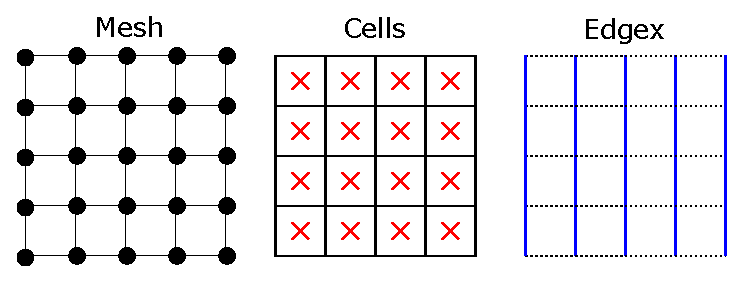
\includegraphics{images/mesh.pdf}}
\end{center}
\begin{columns}
\begin{column}{6.5cm}
%    \fontsize{11}{11}\selectfont
  \begin{lstlisting}[frame=single]
mesh : cart
mesh entities : cell, edgex
computation domains :
  d1 in cell
  d2 in edgex
stencil shapes : 
  ncc from cell to cell
  nce from cell to edgex
  nec from edgex to cell
\end{lstlisting}
\end{column}
\begin{column}{5.5cm}
\begin{itemize}
\item A cartesian mesh is used
\item Two kinds of mesh entities are declared onto it
\item Two computations domains, one for each entity type
\item Three stencil shapes (neighborhood from mesh entity to mesh entity)
\end{itemize}
\end{column}
\end{columns}
\end{frame}
%-------------------------------------------------------------
\begin{frame}[fragile]
\frametitle{The MSL language: quantity}
\begin{columns}
\begin{column}{5cm}
\begin{lstlisting}[frame=single]
quantity :
  A,cell
  B,cell
  C,edgex
  D,cell
  E,cell
  F,cell
  G,cell
  H,edgex
  I,cell
  J,cell
scalar : mu, tau
\end{lstlisting}
\end{column}
\begin{column}{6cm}
\begin{itemize}
\item A is a quantity applied onto cell
\item C is a quantity applied onto edgex
\item mu and tau are scalar values
\end{itemize}
\end{column}
\end{columns}
\end{frame}
%-------------------------------------------------------------
\begin{frame}[fragile]
\frametitle{The MSL language: time and computations}
\begin{columns}
\begin{column}{6cm}
\begin{lstlisting}[frame=single]
time : 500
computations :
  B[d1] = k0({tau},{A})
  C[d2] = k1({},{B[nce]})
  D[d1] = k2({},{C})
  E[d1] = k3({},{C})
  F[d1] = k4({},{D,C[nec]})
  G[d1] = k0({mu,tau},{E})
  H[d2] = k6({},{F})
  I[d1] = k7({},{G,H})
  J[d1] = k8({mu},{I[ncc]})
\end{lstlisting}
\end{column}
\begin{column}{5cm}
\begin{itemize}
\item The time loop is composed of 500 iterations.
\item J is written
\item onto the computation domain d1,
\item by the computation k8,
\item which read the scalar mu
\item and the quantity I,
\item which is accessed with the neighborhood ncc.
\end{itemize}
\end{column}
\end{columns}
\end{frame}
%-------------------------------------------------------------

%% %-------------------------------------------------------------
%% \section{Multi-Stencil Language : Yet another DSL for stencils !}
%% %-------------------------------------------------------------
%% \begin{frame}
%% \frametitle{Multi-Stencil application}
%% \begin{center}
%% \resizebox{\textwidth}{!}{%
%% \begin{tikzpicture}
%% \def \n {5}
%% \def \radius {3cm}
%% \def \margin {8} % margin in angles, depends on the radius

%%   \node[purp2,align=center] (edp) at ({360/\n * (2 - 1)}:\radius) {Partial Differential Equations\\\scriptsize $\frac{\partial u(x,y,t)}{\partial t} = \frac{\partial^2 u(x,y,t)}{\partial x^2} + \frac{\partial^2 u(x,y,t)}{\partial y^2}$};
%%   \node[progm,align=center,right of=edp,node distance=6cm] (cond) {\scriptsize + specific behavior for\\\scriptsize boundary conditions};
%%   \path[line,dashed] (edp) -- (cond);
%%   \node[purp,align=center] (maillage) at ({360/\n * (1 - 1)}:\radius) {Mesh\\Time iterations};
%%   \path[->] (maillage) edge[<-,thin,shorten <=2pt,shorten >=2pt, bend right=40]  node [fill=white,align=center] {\scriptsize Time and space\\\scriptsize discretization} (edp.east);
%%   \path[] (edp.west) edge[thin,shorten <=2pt,shorten >=2pt, bend right=90]  node [draw,circle,fill=white] (plus) {\scriptsize +} (maillage.west);
%%   \node[purp,align=center, below of=plus, node distance=3.5cm] (sche) {Explicit\\numerical schemes\\\textcolor{red}{stencils}};
%%   \node[progm, text width=11em,align=center,right of=sche,node distance=5.5cm] (expl) {\scriptsize Iterative neighboorhood approximation of the phenomena};
%%   \path[line,dashed] (sche) -- (expl);
%%   \path[line] (plus) -- node [fill=white,align=center] {\scriptsize Numerical methods\\\scriptsize Finite difference/volume/elment} (sche);
%% \end{tikzpicture}
%% }
%% \end{center}
%% \end{frame}
%% %----------------
%% \begin{frame}
%% \frametitle{Multi-Stencil Language : Yet another DSL for stencils !}
%% \begin{block}{Inputs}
%% follow a descriptive grammar to simply declare
%% \begin{itemize}
%% \item the sequential order of computations
%% \item what is read and written by each computation
%% \item with or without a neighborhood access (stencil)
%% \end{itemize}
%% \end{block}
%% \begin{block}{Outputs}
%% \begin{itemize}
%% \item parallel pattern of the multi-stencil application
%% \item hybrid parallelism included: data and task parallelism
%% \item choice of parallel languages (MPI, OpenMP 3.x/4.x, SkelGIS etc.)
%% \item end-users have to fill computation functions into this pattern
%% \end{itemize}
%% \end{block}
%% \end{frame}
%% %----------------
%% \begin{frame}
%% \frametitle{Multi-Stencil Language : Yet another DSL for stencils !}
%% \begin{itemize}
%% \item Choosen abstraction level
%% \begin{itemize}
%% \item mesh-agnostic description language
%% \begin{itemize}
%% \item should be usable for unstructured, Cartesian, curvilinear meshes
%% \end{itemize}
%% \item description concerns splited from implementation concerns
%% \begin{itemize}
%% \item usable with many different parallel libraries or languages back-ends
%% \end{itemize}
%% \end{itemize}
%% \item Choosen programming models for back-end
%% \begin{itemize}
%% \item Component programming model (maintainability, portability and composability)
%% \item Task scheduling model (portability and efficiency)
%% \end{itemize}
%% \item Reuse of existing languages and DSLs
%% \begin{itemize}
%% \item Use of a Distributed Data Structure DSeL (C++,MPI) : SkelGIS
%% \item MPI and OpenMP (3.x and 4.x)
%% \end{itemize}
%% \end{itemize}
%% \end{frame}
%% %-------------------------------------------------------------

%-------------------------------------------------------------
\section{From DSL to Component Assembly}
%-------------------------------------------------------------
%----------------
\begin{frame}
\frametitle{Data and Task parallelism}
\begin{block}{Synchronizations}
When a computation read a data, using a stencil shape, that has been written by a previous computation.
\end{block}

$\Gamma = [c_0,c_1,c_2,c_3,c_4,c_5,c_6,c_7,c_8]$\\
$\hookrightarrow [c_0,sync_1,c_1,c_2,c_3,sync_4,c_4,c_5,c_6,c_7,sync_8,c_8]$

\medskip

\begin{block}{Dependency graph}
%\begin{enumerate}
Node: a computation or a synchronization\\
Edge: a direct data dependency (Read / Write)
\end{block}

\begin{center}
\begin{tikzpicture}[shorten >=1pt, node distance=2cm, on grid, auto]
   \node (c0) at (0,0) {$c_0$};
   \node[right=1 of c0] (sy1) {$sync_1$};
   \node[right=1 of sy1] (c1) {$c_1$};
   \node[above right=1 of c1] (c2) {$c_2$};
   \node[below right=1 of c1] (c3) {$c_3$};
   \node[right=1 of c2] (sy4) {$sync_4$};
   \node[right=1 of c3] (c5) {$c_5$};
   \node[right=1 of sy4] (c4) {$c_4$};
   \node[right=1 of c4] (c6) {$c_6$};
   \node[below right=1 of c6] (c7) {$c_7$};
   \node[right=1 of c7] (sy8) {$sync_8$};
   \node[right=1 of sy8] (c8) {$c_8$};
 
  \path[->]
    (c0) edge node {} (sy1)
    (sy1) edge node {} (c1)
    (c1)  edge node {} (c2)
          edge node {} (c3)
    (c2) edge node {} (sy4)
    (sy4) edge node {} (c4)
    (c4) edge node {} (c6)
    (c3) edge node {} (c5)
    (c5) edge node {} (c7)
    (c6) edge node {} (c7)
    (c7) edge node {} (sy8)
    (sy8) edge node {} (c8);
\end{tikzpicture}
\end{center}

\begin{center}
\textcolor{red}{Static} or \textcolor{red}{dynamic} scheduling ?
\end{center}
\end{frame}
%----------------
%----------------
\begin{frame}
\frametitle{MSL to Component-based runtime}
\begin{block}{Ready-to-fill parallel pattern}
\begin{itemize}
\item Data parallelism
\begin{itemize}
\item External distributed data structure
\item Automatic detection of synchronizations
\end{itemize}
\item Task parallelism (mid-grain)
\begin{itemize}
\item Static scheduling at the assembly level 
\item Dynamic scheduling within a driver component
  \begin{itemize}
  \item OpenMP task (For loop also available)
  \end{itemize}
\end{itemize}
\end{itemize}
\end{block}
The fine grain task parallelism is left to other languages: 
\begin{itemize}
\item OpenMP in the kernels
\item Kernels generated by stencil compilers
  \begin{itemize}
  \item Pochoir, PATUS, Liszt etc.
  \end{itemize}
\end{itemize}
\end{frame}
%----------------
%-------------------------------------------------------------
\begin{frame}
\frametitle{Component Assembly Runtime Template}
A data parallel/task parallel component assembly.\vspace{-0.2em}

\begin{center}
\begin{tikzpicture}[remember picture]
  \node[rectangle,rounded corners=3pt,thick,inner sep=5pt,draw=black,dotted] (proc) {
    \begin{tikzpicture}[shorten >=1pt, node distance=2cm, on grid, auto]
     \node[component,solid,draw=black] (D) at (0,0) {$Driver$};
     \node[provide,scale=0.5,solid] (Dp) at (-1,0) {};
     \node[solid] (Ds) at (-1.5,0) {start};
     \node[use,scale=0.5,solid,right=1.5cm of D] (Du1) {};
     \node[use,scale=0.5,solid,below=1.75cm of D] (Du2) {};
     \node[use,scale=0.5,solid,below=0.8cm of Du1] (Du3) {$m$};

     \node[provide,scale=0.5,solid,below=0.15 of Du2] (Tp) {};
     \node[component,solid,below=1.6cm of Tp] (T) {$Time$};
     \node[use,scale=0.5,solid,right=1cm of T] (Tu) {};
     \node[solid,left=0.8cm of T] (tt) {$T$};

     \node[provide,scale=0.5,solid,right=0.15 of Tu] (Cp) {};
     \node[component,solid,right=2cm of Cp] (C) {$Scheduler$};
     \node[use,scale=0.5,solid,above=0.8cm of C] (Cu) {};
     \node[use,scale=0.5,solid,right=1.5cm of C] (Cu2) {};
     \node[use,scale=0.5,solid,below=0.8cm of Cu2] (Cu3) {};
     \node[use,scale=0.5,solid,below=0.8cm of Cu3] (Cu4) {};
     \node[solid,right=0.2cm of Cu] (star) {$*$};
     %\node[solid,right=1.5cm of C] (gamma) {$\Gamma$};

     \node[solid,below=1cm of C] (calc) {$\Gamma_{sync}$, $\Gamma_{dep}$};

     \node[provide,scale=0.5,solid,right=0.15 of Cu2] (k0p) {};
     \node[component,solid,right=1.5cm of k0p] (k0) {$k_0$};

     \node[provide,scale=0.5,solid,right=0.15 of Cu3] (k0sp) {};
     \node[component,solid,right=1.5cm of k0sp] (k0s) {$k_{0;1}^{sync}$};

     \node[provide,scale=0.5,solid,right=0.15 of Cu4] (kotherp) {};
     \node[component,solid,right=1.5cm of kotherp] (kother) {$\dots$};

     \node[provide,scale=0.5,solid,below right=0.2 of Du3] (Datap1) {};
     \node[provide,scale=0.5,solid,above=0.15 of Cu] (Datap2) {};
     \node[component,solid,double,above=0.8cm of Datap2] (Data) {$Quantity$};
     \node[use,scale=0.5,solid,above=0.8cm of Data] (Datau) {};
     \node[solid,left=1.5cm of Data] (delta) {$\Delta,\mathcal{D}$};
     %\node[mpi,scale=0.8,rounded corners=0pt,solid,right=1cm of Data] (mpidata) {};
     %\node[solid,above=0.2cm of mpidata] (star2) {$*$};

     \node[provide,scale=0.5,solid,right=0.15 of Du1] (DDSp1) {};
     \node[provide,scale=0.5,solid,above=0.15 of Datau] (DDSp2) {};
     \node[component,solid,above=0.8cm of DDSp2] (DDS) {$DDS$};
     \node[solid,right=1.2cm of DDS] (m) {$\mathcal{M},\mathcal{E}$};
   
    \path[-]
      (Dp) edge [solid] node {} (D)
      (D) edge [solid] node {} (Du1)
          edge [solid] node {} (Du2)
          edge [solid] node {} (Du3)
      (DDSp1) edge [solid] node {} (DDS)
      (Tp) edge [solid] node {} (T)
      (T)  edge [solid] node {} (Tu)
      (Cp) edge [solid] node {} (C)
      (C) edge [solid] node {} (Cu)
      (Datap2) edge [solid] node {} (Data)
      (Datap1) edge [solid] node {} (Data)
      (Data) edge [solid] node {} (Datau)
      (DDSp2) edge [solid] node {} (DDS)
      (C)  edge [solid] node {} (Cu2)
          edge [solid] node {} (Cu3)
          edge [solid] node {} (Cu4)
      (Cu2)  edge [solid] node {} (k0p)
      (k0p)  edge [solid] node {} (k0)
      (Cu3)  edge [solid] node {} (k0sp)
      (k0sp)  edge [solid] node {} (k0s)
      (Cu4)  edge [solid] node {} (kotherp)
      (kotherp)  edge [solid] node {} (kother);
    \end{tikzpicture}
    };
    \node[mpi,scale=0.8,rounded corners=0pt,solid,right=4cm of Data] (mpidata) {};
    \node[solid,above=0.1cm of mpidata] (star2) {$*$};
    \node[solid,above=3.2cm of proc.west,anchor=west] (core) {\textit{\tiny{Applied on each resource}}};
    \path[-]
      (Data.east) edge node {} (mpidata);
  \end{tikzpicture}
\end{center}
{\fontsize{8}{8}\selectfont DDS: Distributed Data Structure (using SkelGIS)\par}
\end{frame}
%% %-------------------------------------------------------------
%% \begin{frame}
%% \frametitle{What is produced ?}
%% \begin{block}{Implementation}
%% \begin{itemize}
%% \item DDS + Quantity + $k_{*}^{sync}$ = written components using SkelGIS (distributed memory, MPI)
%% \item Scheduler = Serie-Parallel graph of $\Gamma_{dep}$ (OpenMP 3.0)
%% \item Time + Scheduler = generated components
%% \item $k_i$ = empty components to write
%% \end{itemize}
%% \end{block}

%% \begin{block}{Separation of concerns}
%% \begin{itemize}
%% \item numerician (MSL)
%% \item computer engineer (K)
%% \item HPC engineer (DDS, quantity, $k_{*}^{sync}$ etc.)
%% \item DSL designer (component assembly + generated components)
%% \end{itemize}
%% \end{block}
%% \end{frame}
%% %-------------------------------------------------------------

%% \begin{frame}
%% \frametitle{Series-Parallel Tree}
%% \small\textit{Valdes \& Al, The Recognition of Series Parallel Digraphs, STOC '79}
%% \normalsize
%% \begin{columns}
%% \begin{column}{.48\textwidth}
%% \begin{center}
%% \resizebox{\textwidth}{!}{%
%% \begin{tikzpicture}[shorten >=1pt, node distance=2cm, on grid, auto]
%%    \node[] (s0)    at (0,0) {$\mathcal{S}$};
   
%%    \node[] (c0)    at (-3,1) {$c_0$};
%%    \node[] (star1) at (-2,1) {$sync_1$};
%%    \node[] (c1)    at (-1,1) {$c_1$};
%%    \node[] (p0)    at ( 0,1) {$\mathcal{P}$};
%%    \node[] (c7)    at ( 1,1) {$c_7$};
%%    \node[] (star8) at ( 2,1) {$sync_8$};
%%    \node[] (c8)    at ( 3,1) {$c_8$};

%%    \node[] (s1)    at (-1,2) {$\mathcal{S}$};
%%    \node[] (s2)    at (1,2) {$\mathcal{S}$};
   
%%    \node[] (c2)    at (-3,3) {$c_2$};
%%    \node[] (star4) at (-2,3) {$sync_4$};
%%    \node[] (c4)    at (-1,3) {$c_4$};
%%    \node[] (c6)    at ( 0,3) {$c_6$};
%%    \node[] (c3)    at ( 1,3) {$c_3$};
%%    \node[] (c5)    at ( 2,3) {$c_5$};

 
%%   \path[->]
%%     (s0) edge node {} (c0)
%%          edge node {} (star1)
%%          edge node {} (c1)
%%          edge node {} (p0)
%%          edge node {} (c7)
%%          edge node {} (star8)
%%          edge node {} (c8)
%%     (p0) edge node {} (s1)
%%          edge node {} (s2)
%%     (s1) edge node {} (c2)
%%          edge node {} (star4)
%%          edge node {} (c4)
%%          edge node {} (c4)
%%          edge node {} (c6)
%%     (s2) edge node {} (c3)
%%          edge node {} (c5);
%%   \end{tikzpicture}
%%   }
%% \end{center}
%% \end{column}
%% \begin{column}{.52\textwidth}

%% \end{column}
%% \end{columns}
%% \end{frame}
%% %----------------

%% %----------------
%% \begin{frame}
%% \frametitle{Series-Parallel Tree}
%% \small\textit{Valdes \& Al, The Recognition of Series Parallel Digraphs, STOC '79}
%% \normalsize
%% \begin{columns}
%% \begin{column}{.48\textwidth}
%% \begin{center}
%% \resizebox{\textwidth}{!}{%
%% \begin{tikzpicture}[shorten >=1pt, node distance=2cm, on grid, auto]
%%    \node[] (s0)    at (0,0) {$\mathcal{S}$};
   
%%    \node[] (c0)    at (-3,1) {$c_0$};
%%    \node[] (star1) at (-2,1) {$sync_1$};
%%    \node[] (c1)    at (-1,1) {$c_1$};
%%    \node[] (p0)    at ( 0,1) {$\mathcal{P}$};
%%    \node[] (c7)    at ( 1,1) {$c_7$};
%%    \node[] (star8) at ( 2,1) {$sync_8$};
%%    \node[] (c8)    at ( 3,1) {$c_8$};

%%    \node[] (s1)    at (-1,2) {$\mathcal{S}$};
%%    \node[] (s2)    at (1,2) {$\mathcal{S}$};
   
%%    \node[] (c2)    at (-3,3) {$c_2$};
%%    \node[] (star4) at (-2,3) {$sync_4$};
%%    \node[] (c4)    at (-1,3) {$c_4$};
%%    \node[] (c6)    at ( 0,3) {$c_6$};
%%    \node[] (c3)    at ( 1,3) {\textcolor{red}{$c_3;c_5$}};
%%    %\node[] (c5)    at ( 2,3) {$c_5$};

 
%%   \path[->]
%%     (s0) edge node {} (c0)
%%          edge node {} (star1)
%%          edge node {} (c1)
%%          edge node {} (p0)
%%          edge node {} (c7)
%%          edge node {} (star8)
%%          edge node {} (c8)
%%     (p0) edge node {} (s1)
%%          edge node {} (s2)
%%     (s1) edge node {} (c2)
%%          edge node {} (star4)
%%          edge node {} (c4)
%%          edge node {} (c4)
%%          edge node {} (c6)
%%     (s2) edge node {} (c3);
%%   \end{tikzpicture}
%%   }
%% \end{center}
%% \end{column}
%% \begin{column}{.52\textwidth}
%% \end{column}
%% \end{columns}
%% Loop fusion optimization possible
%% \end{frame}
%% %----------------

%% %----------------
%% \begin{frame}
%% \frametitle{Series-Parallel Tree}
%% \small\textit{Valdes \& Al, The Recognition of Series Parallel Digraphs, STOC '79}
%% \normalsize
%% \begin{columns}
%% \begin{column}{.48\textwidth}
%% \begin{center}
%% \resizebox{\textwidth}{!}{%
%% \begin{tikzpicture}[shorten >=1pt, node distance=2cm, on grid, auto]
%%    \node[] (s0)    at (0,0) {$\mathcal{S}$};
   
%%    \node[] (c0)    at (-3,1) {$c_0$};
%%    \node[] (star1) at (-2,1) {$sync_1$};
%%    \node[] (c1)    at (-1,1) {$c_1$};
%%    \node[] (p0)    at ( 0,1) {$\mathcal{P}$};
%%    \node[] (c7)    at ( 1,1) {$c_7$};
%%    \node[] (star8) at ( 2,1) {$sync_8$};
%%    \node[] (c8)    at ( 3,1) {$c_8$};

%%    \node[] (s1)    at (-1,2) {$\mathcal{S}$};
%%    \node[] (s2)    at (1,2) {$\mathcal{S}$};
   
%%    \node[] (c2)    at (-3,3) {$c_2$};
%%    \node[] (star4) at (-2,3) {$sync_4$};
%%    \node[] (c4)    at (-1,3) {$c_4$};
%%    \node[] (c6)    at ( 0,3) {$c_6$};
%%    \node[] (c3)    at ( 1,3) {\textcolor{red}{$c_3;c_5$}};
%%    %\node[] (c5)    at ( 2,3) {$c_5$};

 
%%   \path[->]
%%     (s0) edge node {} (c0)
%%          edge node {} (star1)
%%          edge node {} (c1)
%%          edge node {} (p0)
%%          edge node {} (c7)
%%          edge node {} (star8)
%%          edge node {} (c8)
%%     (p0) edge node {} (s1)
%%          edge node {} (s2)
%%     (s1) edge node {} (c2)
%%          edge node {} (star4)
%%          edge node {} (c4)
%%          edge node {} (c4)
%%          edge node {} (c6)
%%     (s2) edge node {} (c3);
%%   \end{tikzpicture}
%%   }
%% \end{center}
%% \end{column}
%% \begin{column}{.52\textwidth}
%% \begin{block}{Specific components}
%% \begin{itemize}
%% \item $SEQ$ to directly replace $\mathcal{S}$ nodes
%% \item $PAR$ to directly replace $\mathcal{P}$ nodes
%% \item $SYNC$ for synchronizations
%% \item $K$ for computation kernels
%% \end{itemize}
%% \end{block}
%% \end{column}
%% \end{columns}
%% Loop fusion optimization possible
%% \end{frame}
%% %----------------

%% %-------------------------------------------------------------
%% \section{Implementation}
%% %-------------------------------------------------------------
%% \begin{frame}
%% \frametitle{Component models}
%% \begin{itemize}
%% \item Black box with code
%% \item Use/provide interfaces
%% \item Improve code reuse (productivity)
%% \item Improve separation of concerns (maintainability and portability)
%% \item Improve composability of applications
%% \end{itemize}
%% \begin{center}
%% \begin{tikzpicture}[remember picture]
%%   \node[component,solid] (A) at (0,0) {A};
%%   \node[component,solid,right=5cm of A] (B) {B};
%%   \node[use,scale=0.5,solid,right=1.5cm of A] (Au) {};
%%   \node[provide,scale=0.5,solid,left=1.5cm of B] (Bp) {};
%%   \path[-]
%%     (A) edge node {} (Au)
%%     (Bp) edge node {} (B);
%% \end{tikzpicture}

%% \bigskip
%% \begin{tikzpicture}[remember picture]
%%   \node[component,solid] (A) at (0,0) {A};
%%   \node[use,scale=0.5,solid,right=1cm of A] (Au) {};
%%   \node[provide,scale=0.5,solid,right=0.01cm of Au] (Bp) {};
%%   \node[component,solid,right=1cm of Bp] (B) {B};
%%   \path[-]
%%     (A) edge node {} (Au)
%%     (Bp) edge node {} (B);
%% \end{tikzpicture}

%% \medskip
%% Components A and B into a component assembly
%% \end{center}
%% \end{frame}


%-------------------------------------------------------------
\section{Evaluations}
%----------------
\begin{frame}
\frametitle{Evaluations}
\begin{block}{Application}
\begin{itemize}
\item FullSWOF2D: developed at the MAPMO, Université d'Orléans
\item Solve the shallow-water equations using a finite volume method
\item Cartesian mesh
\item 3 mesh entities, 7 computation domains, 48 quantities
\item 98 computations (32 stencils, 66 local kernels)
\end{itemize}
\end{block}
\begin{block}{Machines}
\begin{itemize}
\item Thin nodes TGCC Curie
\item 2 CPU, 8 cores, Sandy Bridge EP (E5-2680) 2.7 GHz, 64 GB
\item OpenMPI and gcc 4.9
\end{itemize}
\end{block}
\end{frame}
%----------------
%-------------------------------------------------------------
\begin{frame}
\frametitle{Data Parallelization: Weak and Strong Scaling}
\begin{columns}
\begin{column}{6cm}
\resizebox{6cm}{!}{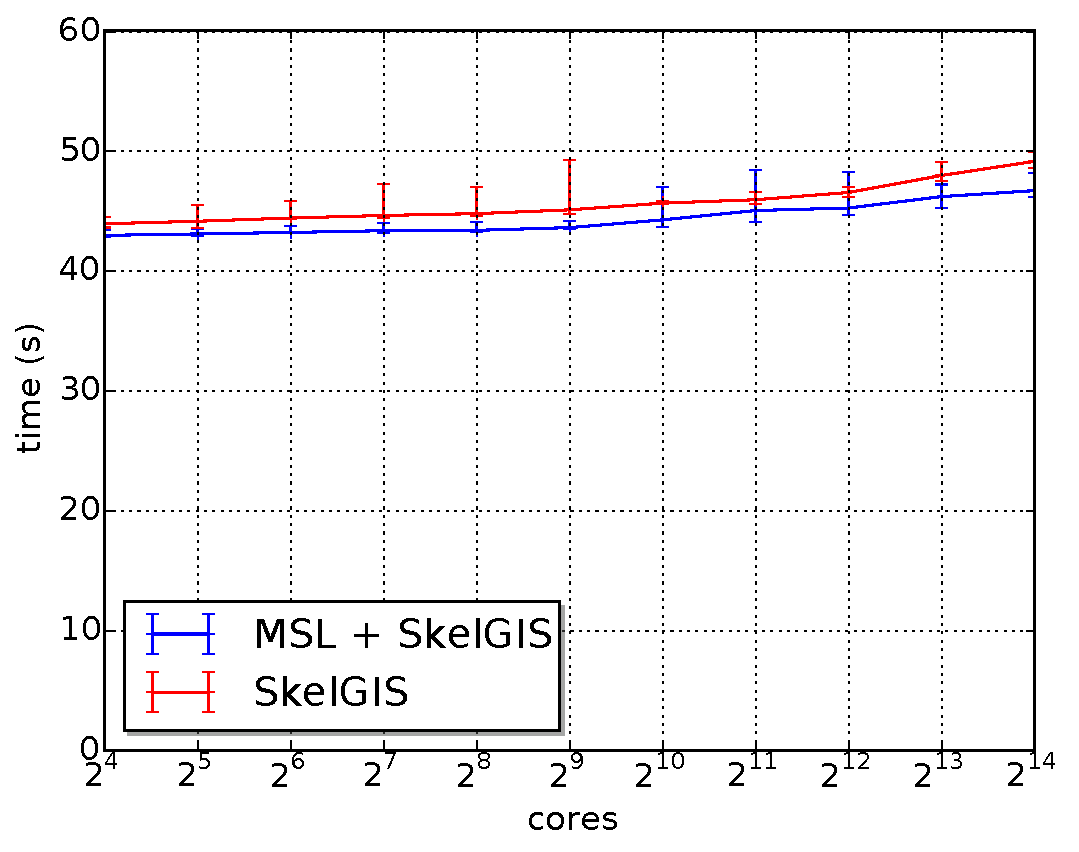
\includegraphics{images/median_weak.pdf}}
\begin{center}
\vspace{-1em}
  Weak Scaling\\
  400x400 domain/core
\end{center}
\end{column}
\begin{column}{6cm}
\resizebox{6cm}{!}{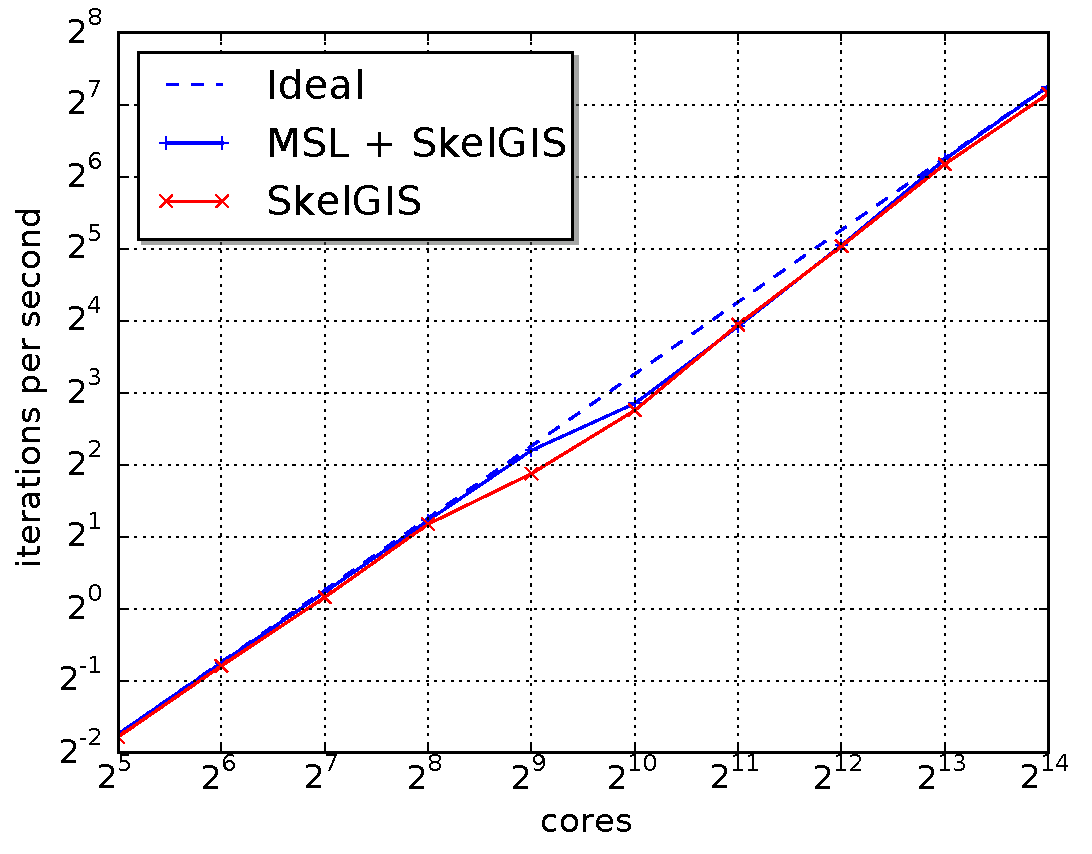
\includegraphics{images/median_strong.pdf}}
\begin{center}
\vspace{-1em}
  Strong Scaling\\
  10k x 10k domaine
\end{center}
\end{column}
\end{columns}
\bigskip
\begin{center}
  \textbf{No overhead introduced by components}
\end{center}
\end{frame}
%-------------------------------------------------------------
\begin{frame}
\frametitle{Data Paralization to Hybrid Parallization: Strong Scaling}
\begin{columns}
\begin{column}{6cm}
  \resizebox{6cm}{!}{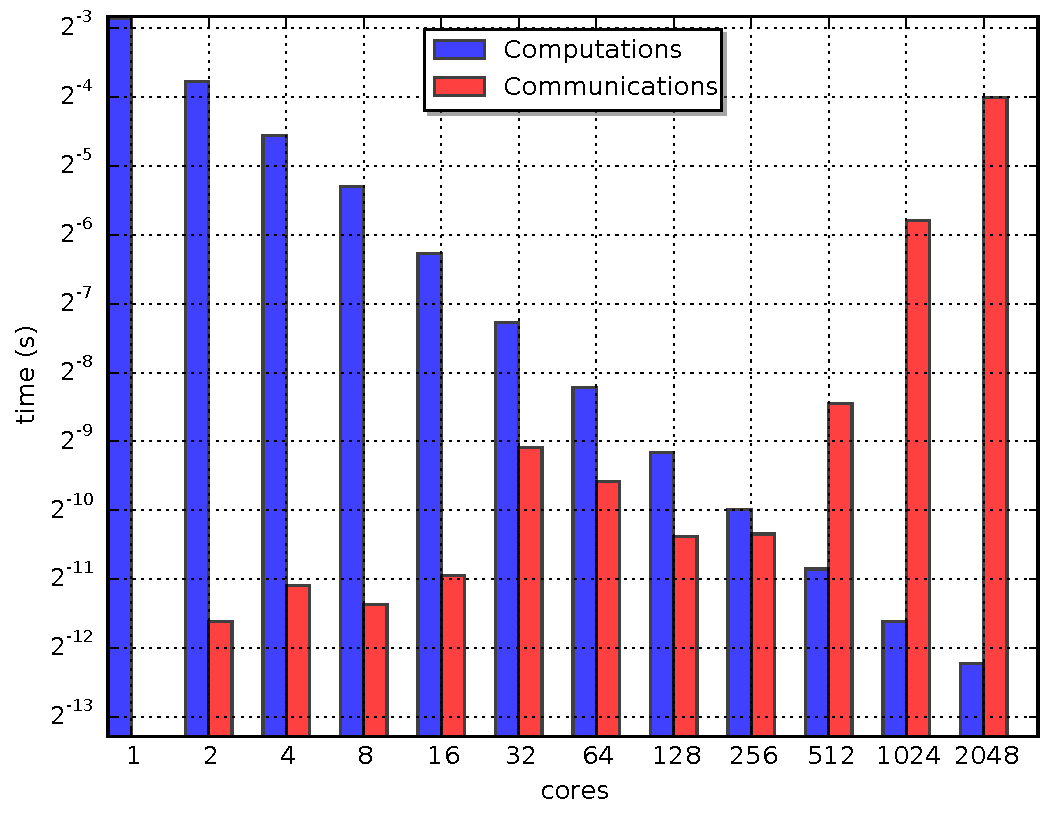
\includegraphics{images/times.pdf}}
  \begin{center}
\vspace{-1em}\small    Data Parallelization    
  \end{center}
\end{column}
\begin{column}{6cm}
\resizebox{6cm}{!}{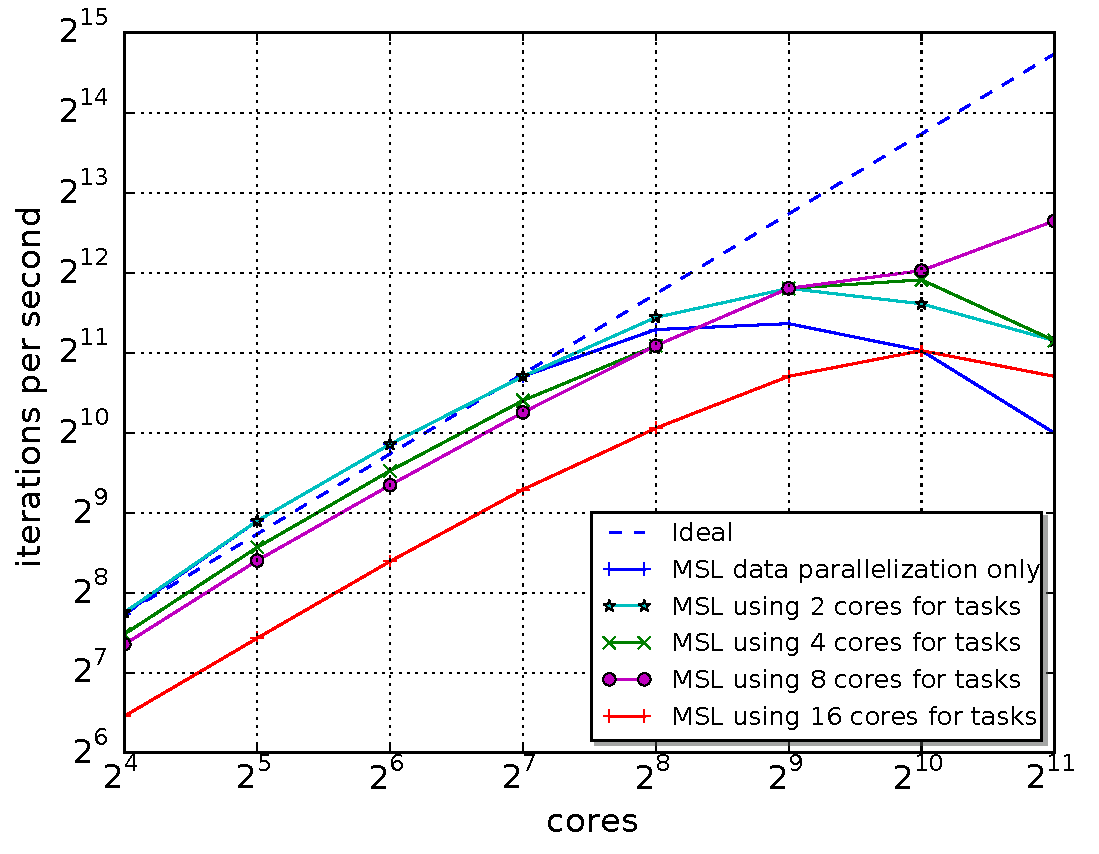
\includegraphics{images/base_close_median.pdf}}
\begin{center}
\vspace{-1em}\small  Data and Hybrid Parallelizations
\end{center}
\end{column}
\end{columns}
\bigskip
\begin{center}
{\small
  \begin{tabular}{|c|c|c|c|c|c|c|c|c|}
    \hline 
   Parallelism Level & 1 & 2 & 3 & 4 & 6 & 10 & 12 & 16\\
   \hline
   Frequency & 2 & 1 & 3 & 5 & 3 & 1 & 1 & 2\\
   \hline
 \end{tabular}
 \\
 Task graph analysis
}
\end{center}
\end{frame}
%-------------------------------------------------------------


%-------------------------------------------------------------
\section{Conclusion}
%-------------------------------------------------------------
%\subsection{Conclusion and perspectives}
\begin{frame}
\frametitle{Conclusion and Future Work}
\begin{block}{Conclusion}
\begin{itemize}
\item A DSL for Multi-Stencil applications (MSL)
\item The generation of a component based runtime, including scheduling
\begin{itemize}
\item Data parallelism
\item Task parallelism
\end{itemize}
\item Evaluation on Curie: no overhead introduced 
\end{itemize}
\end{block}

\begin{block}{Future Work}
  \begin{itemize}
  \item Language improvement (convergence criteria, reduction etc.)
  \item OpenMP 3 inside kernels
  \item CPU+GPGPUs using stencil compilers (Pochoir, PATUS etc.)
$\hookrightarrow$ Show portability, maintainability introduced by components

  \end{itemize}
\end{block}
\end{frame}
%-------------------------------------------------------------


%% %-------------------------------------------------------------
%% \begin{frame}
%% \frametitle{Conclusion}
%% \begin{block}{Work in progress}
%% \begin{itemize}
%% \item Different types of scheduling and back-end in MSL
%% \item Combine MSL implementation choices to an energy-aware framework
%% \item New programming model back-end for MSL: combining component models and task models (Ph.D. Jérôme Richard)
%% \end{itemize}
%% \end{block}
%% \begin{block}{Collaborations}
%% \begin{itemize}
%% \item More application cases
%% \item Back-end programming model: component models and task scheduling (Components in OmpSs ?)
%% \item DSLs interoperability
%% \end{itemize}
%% \end{block}
%% \end{frame}
%-------------------------------------------------------------

% \begin{withoutheadline}
% \begin{frame}{}
% \begin{center}
% \huge Thank You !
% \end{center}
% \end{frame}
% \end{withoutheadline}

%----------------
%% \begin{frame}
%% \frametitle{MSL to Component-based runtime}
%% \begin{center}
%% \begin{tikzpicture}[remember picture]
%%   \node[rectangle,rounded corners=3pt,thick,inner sep=5pt,draw=black,dotted] (proc) {
%%     \begin{tikzpicture}[shorten >=1pt, node distance=2cm, on grid, auto]
%%      \node[component,solid] (D) at (0,0) {$Driver$};
%%      \node[provide,scale=0.5,solid] (Dp) at (-1,0) {};
%%      \node[solid] (Ds) at (-1.5,0) {start};
%%      \node[use,scale=0.5,solid,right=1.5cm of D] (Du1) {};
%%      \node[use,scale=0.5,solid,below=1.75cm of D] (Du2) {};
%%      \node[use,scale=0.5,solid,below=0.8cm of Du1] (Du3) {$m$};

%%      \node[provide,scale=0.5,solid,below=0.15 of Du2] (Tp) {};
%%      \node[component,solid,below=1.6cm of Tp] (T) {$Time$};
%%      \node[use,scale=0.5,solid,right=1cm of T] (Tu) {};

%%      \node[provide,scale=0.5,solid,right=0.15 of Tu] (Sp) {};
%%      \node[component,solid,right=1.5cm of Sp] (S) {$Scheduling$};
%%      \node[use,scale=0.5,solid,right=1.5cm of S] (Su) {};

%%      \node[provide,scale=0.5,solid,right=0.15 of Su] (Cp) {};
%%      \node[component,solid,double,right=2cm of Cp] (C) {$Kernel$};
%%      \node[use,scale=0.5,solid,above=0.8cm of C] (Cu) {};

%%      \node[provide,scale=0.5,solid,below right=0.2 of Du3] (Datap1) {};
%%      \node[provide,scale=0.5,solid,above=0.15 of Cu] (Datap2) {};
%%      \node[component,solid,double,above=0.8cm of Datap2] (Data) {$Data$};
%%      \node[use,scale=0.5,solid,above=0.8cm of Data] (Datau) {};

%%      \node[provide,scale=0.5,solid,right=0.15 of Du1] (DDSp1) {};
%%      \node[provide,scale=0.5,solid,above=0.15 of Datau] (DDSp2) {};
%%      \node[component,solid,above=0.8cm of DDSp2] (DDS) {$DDS$};
   
%%     \path[-]
%%       (Dp) edge [solid] node {} (D)
%%       (D) edge [solid] node {} (Du1)
%%           edge [solid] node {} (Du2)
%%           edge [solid] node {} (Du3)
%%       (DDSp1) edge [solid] node {} (DDS)
%%       (Tp) edge [solid] node {} (T)
%%       (T)  edge [solid] node {} (Tu)
%%       (Sp) edge [solid] node {} (S)
%%       (S) edge [solid] node {} (Su)
%%       (Datap2) edge [solid] node {} (Data)
%%       (Datap1) edge [solid] node {} (Data)
%%       (Data) edge [solid] node {} (Datau)
%%       (C) edge [solid] node {} (Cu)
%%       	  edge [solid] node {} (Cp)
%%       (DDSp2) edge [solid] node {} (DDS);
%%     \end{tikzpicture}
%%     };
%%     \node[mpi,scale=0.8,rounded corners=0pt,solid,right=0.5cm of proc] (mpidata) {};
%%     \node[solid,above=0.1cm of mpidata] (star2) {$*$};
%%     \node[solid,below=2.5cm of proc.west,anchor=west] (core) {\textit{\tiny{Duplicated on each processor/core}}};
%%     \path[-]
%%       (Data.east) edge node {} (mpidata);
%%   \end{tikzpicture}
%% \end{center}
%% \end{frame}

\end{document}

